\documentclass[10pt]{report}
\usepackage{ctex}
\usepackage[utf8]{inputenc}
\usepackage{amsmath}
\usepackage{amssymb}
\usepackage{xcolor}
\usepackage{graphicx}
\usepackage[margin=0.1cm]{geometry} % 设置页边距为 0.5cm，尽可能扩大可用区域
\usepackage{setspace}
\renewcommand{\baselinestretch}{1} % 设置行间距为单倍行距
\usepackage{float}
\usepackage{wrapfig}
\usepackage[utf8]{inputenc}
\usepackage[T1]{fontenc}
\usepackage{ctex}
\usepackage{amsmath}
\usepackage{amssymb}
\usepackage{xcolor}
\usepackage{graphicx}
\usepackage{float}
\usepackage{lmodern}
\usepackage{mathrsfs}
\usepackage{lipsum}
\usepackage{array} 
\usepackage{tikz}
\usepackage{braket}
\usepackage{adjustbox}
\usepackage{footmisc}
\usepackage{array}
\usepackage{multirow}
\usepackage[table]{xcolor}
\usepackage{amsmath}
\usepackage{tcolorbox}
\usepackage{caption}
\usepackage{tabularx}
\captionsetup[figure]{labelformat=empty} % 设置图标题的标签格式为空，即不显示“图 X”
\usepackage{graphicx}
\tcbuselibrary{listings,breakable}
\usepackage{xcolor}
\setlength{\parindent}{0pt}
\captionsetup[figure]{skip=0pt}
\usepackage{array}
\title{磁滞回线}
\author{张世航}
\begin{document}
	\maketitle
	\section{样品1}
	\subsection{不同频率的磁滞回线}
	\begin{figure}[H]
		\centering
		
\includegraphics[width=0.7\linewidth]{1.1}
		\caption{25Hz}
		\label{fig:1}
	\end{figure}
	\begin{figure}[H]
		\centering
		
\includegraphics[width=0.7\linewidth]{1.2}
		\caption{50Hz}
		\label{fig:2}
	\end{figure}
	\begin{figure}[H]
		\centering
		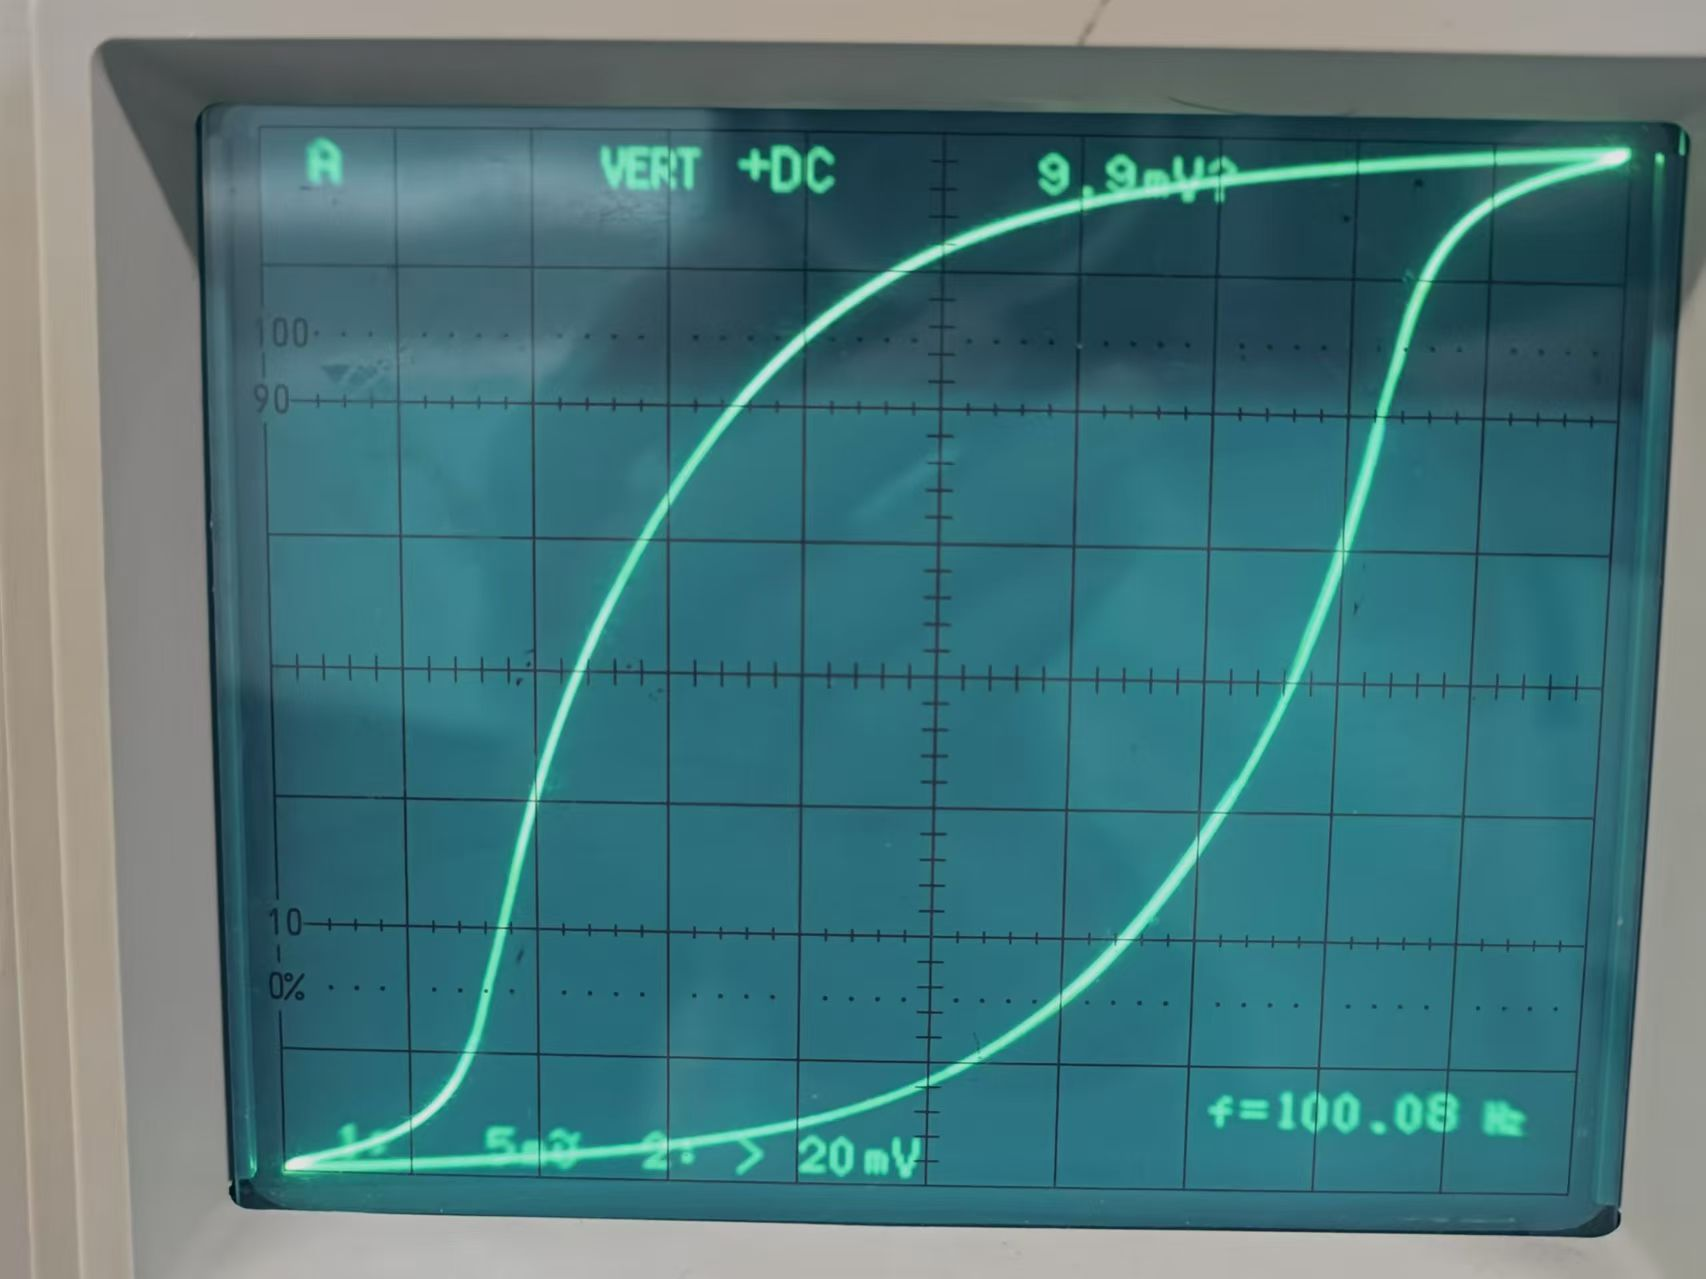
\includegraphics[width=0.7\linewidth]{1.3}
		\caption{100Hz}
		\label{fig:3}
	\end{figure}
	\begin{figure}[H]
		\centering
		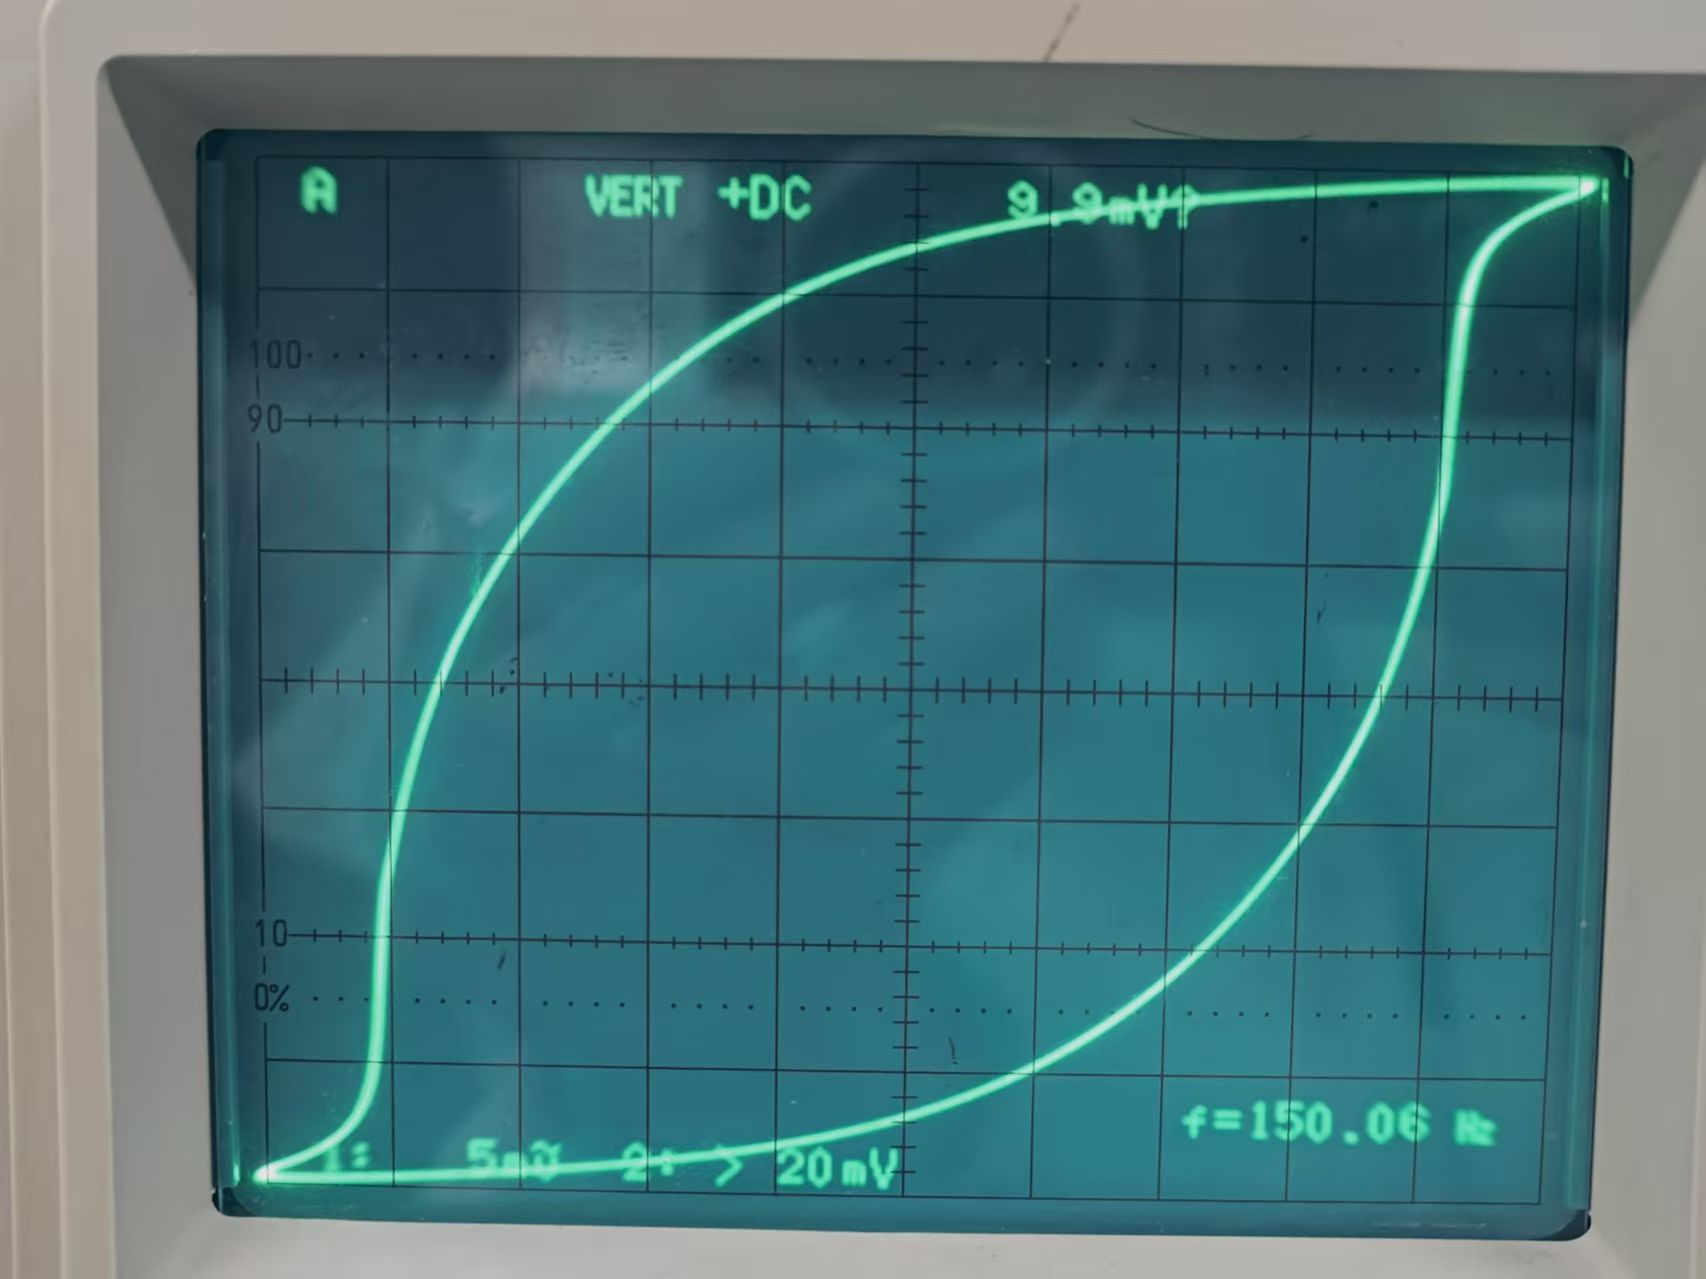
\includegraphics[width=0.7\linewidth]{1.4}
		\caption{150Hz}
		\label{fig:4}
	\end{figure}
	\subsection{基本磁化曲线}
	\begin{table}[H]
		\centering
		\setlength{\extrarowheight}{12pt}  
		\resizebox{0.8\textwidth}{!}{
	\begin{tabular}{|c|c|c|c|c|c|c|c|c|c|c|c|c|}
		\hline
		序号 & 1 & 2 & 3 & 4 & 5 & 6 & 7 & 8 & 9 & 10 & 11 & 12 \\
		\hline
		X格 & 0 & 0.2 & 0.4 & 0.6 & 0.8 & 1.0 & 1.5 & 2.0 & 2.5 & 3.0 & 4.0 & 5.0 \\
		\hline
		H(A/m) &0&  7.69 & 15.38 & 23.07&  30.76&38.46  &57.69&  76.92&  96.15&115.38&153.84 &192.30\\
		\hline
		Y(格) &0&  0.2  &0.46& 0.84 &1.21& 1.6&  2.69 &3.26& 3.56& 3.72& 3.96& 4.02\\
		\hline
		B(mT) & 0& 19.35& 44.52& 81.29& 117.10 &154.84& 260.32 &315.48& 344.52& 360.00 &383.23&
		389.03\\
		\hline
	\end{tabular}
}
\end{table}


	\begin{figure}[H]
		\centering
		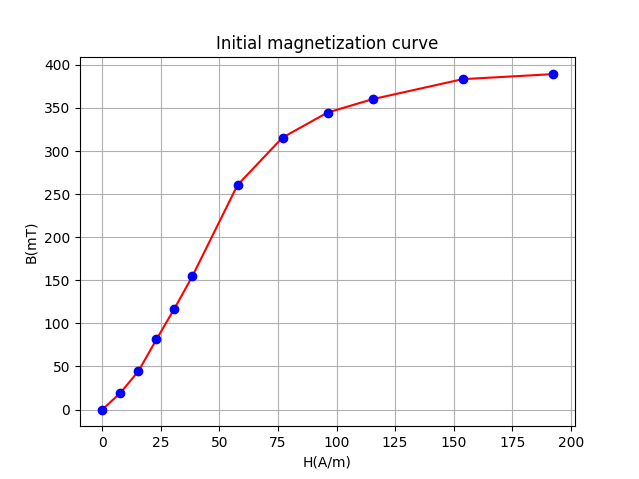
\includegraphics[width=0.7\linewidth]{a}
		\caption{起始磁化曲线}
		\label{fig:5}
	\end{figure}

    \subsection{$\mu_1$}
    \begin{figure}[H]
    	\centering
    	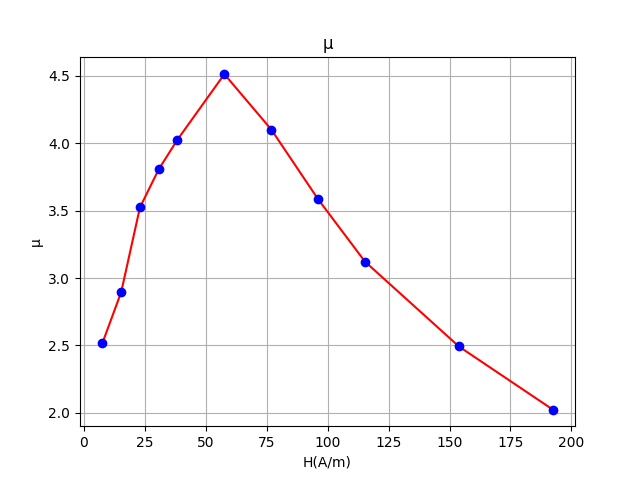
\includegraphics[width=0.7\linewidth]{µ1}
    	\caption{}
    	\label{fig:u1}
    \end{figure}
    
	\subsection{磁滞回线}
	\begin{tabular}{|c|c|c|c|c|c|c|c|c|c|c|c|c|}
		\hline
		序号 & 1 & 2 & 3 & 4 & 5 & 6 & 7 & 8 & 9 & 10 & 11 & 12 \\
		\hline
		X(格) & -5.00 & -4.00 & -3.00 & -2.50 & -2.00 & -1.50 & -1.00 & -0.80 & -0.60 & -0.40 & -0.20 & 0.00 \\
		\hline
		H(A/m) &  -192.31 & -153.85 & -115.38 & -96.15 & -76.92 & -57.69 & -38.46 & -30.77 & -23.08 & -15.38 & -7.69 & 0.00 \\
		\hline
		Y1(格) &-4.02 & -3.87 & -3.20 & -2.01 & -0.58 & 0.79 & 1.72 & 2.06 & 2.31 & 2.53 & 2.76 & 2.88  \\
		\hline
		Y2(格） &-4.02 & -3.96 & -3.85 & -3.76 & -3.67 & -3.55 & -3.44 & -3.32 & -3.27 & -3.13 & -3.04 & -2.89\\
		\hline
		B1(mT） &-389.03 & -374.52 & -309.68 & -194.52 & -56.13 & 76.45 & 166.45 & 199.35 & 223.55 & 244.84 & 267.10 & 278.71  \\
		\hline
		B2(mT) &-389.03 & -383.23 & -372.58 & -363.87 & -355.16 & -343.55 & -332.90 & -321.29 & -316.45 & -302.90 & -294.19 & -279.68\\
		\hline
		X(格） &0.00 & 0.20 & 0.40 & 0.60 & 0.80 & 1.00 & 1.50 & 2.00 & 2.50 & 3.00 & 4.00 & 5.00
		\\
		\hline
		H(A/m) &0.00 & 7.69 & 15.38 & 23.08 & 30.77 & 38.46 & 57.69 & 76.92 & 96.15 & 115.38 & 153.85 & 192.31 \\
		\hline
		Y1(格） & 2.88 & 3.01 & 3.16 & 3.24 & 3.35 & 3.42 & 3.57 & 3.67 & 3.77 & 3.83 & 3.94 & 4.02  \\
		\hline
		Y2(格） &-2.89 & -2.73 & -2.61 & -2.37 & -2.06 & -1.81 & -0.86 & 0.48 & 2.05 & 2.75 & 3.63 & 4.02 \\
		\hline
		B1(mT） &278.71 & 291.29 & 305.81 & 313.55 & 324.19 & 330.97 & 345.48 & 355.16 & 364.84 & 370.65 & 381.29 & 389.03
		\\
		\hline
		B2(mT) & -279.68 & -264.19 & -252.58 & -229.35 & -199.35 & -175.16 & -83.23 & 46.45 & 198.39 & 266.13 & 351.29 & 389.03 \\
		\hline
	\end{tabular}
	\begin{figure}[H]
		\centering
		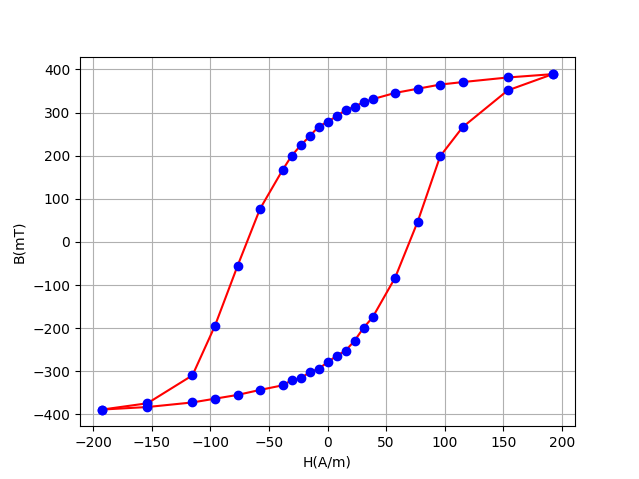
\includegraphics[width=0.7\linewidth]{b}
		\caption{磁滞回线}
		\label{fig:6}
	\end{figure}
	\section{样品2}
	\subsection{不同频率的磁滞回线}
	\begin{figure}[H]
		\centering
		
\includegraphics[width=0.7\linewidth]{2.1}
		\caption{25Hz}
		\label{fig:7}
	\end{figure}
	\begin{figure}[H]
		\centering
		
\includegraphics[width=0.7\linewidth]{2.2}
		\caption{50Hz}
		\label{fig:8}
	\end{figure}
	\begin{figure}[H]
		\centering
		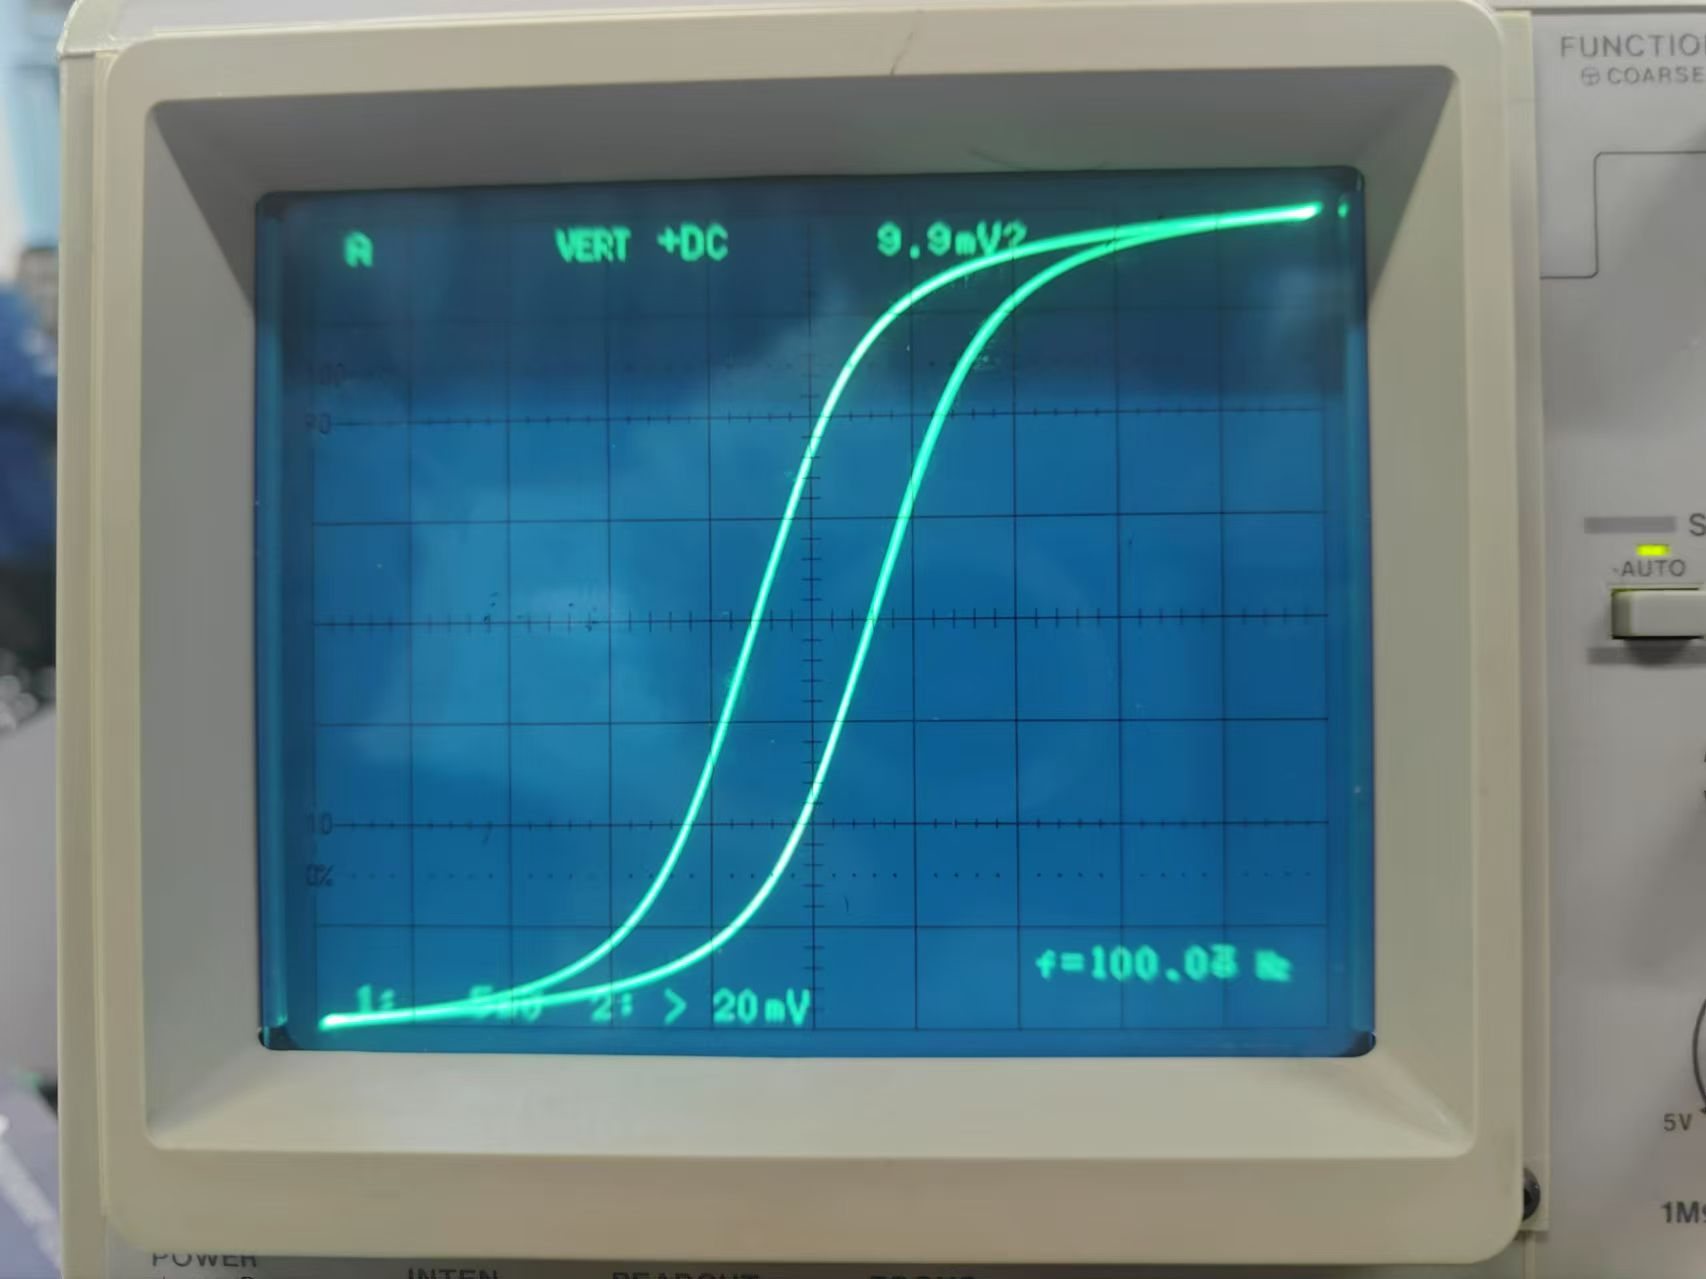
\includegraphics[width=0.7\linewidth]{2.3}
		\caption{100Hz}
		\label{fig:9}
	\end{figure}
	\begin{figure}[H]
		\centering
		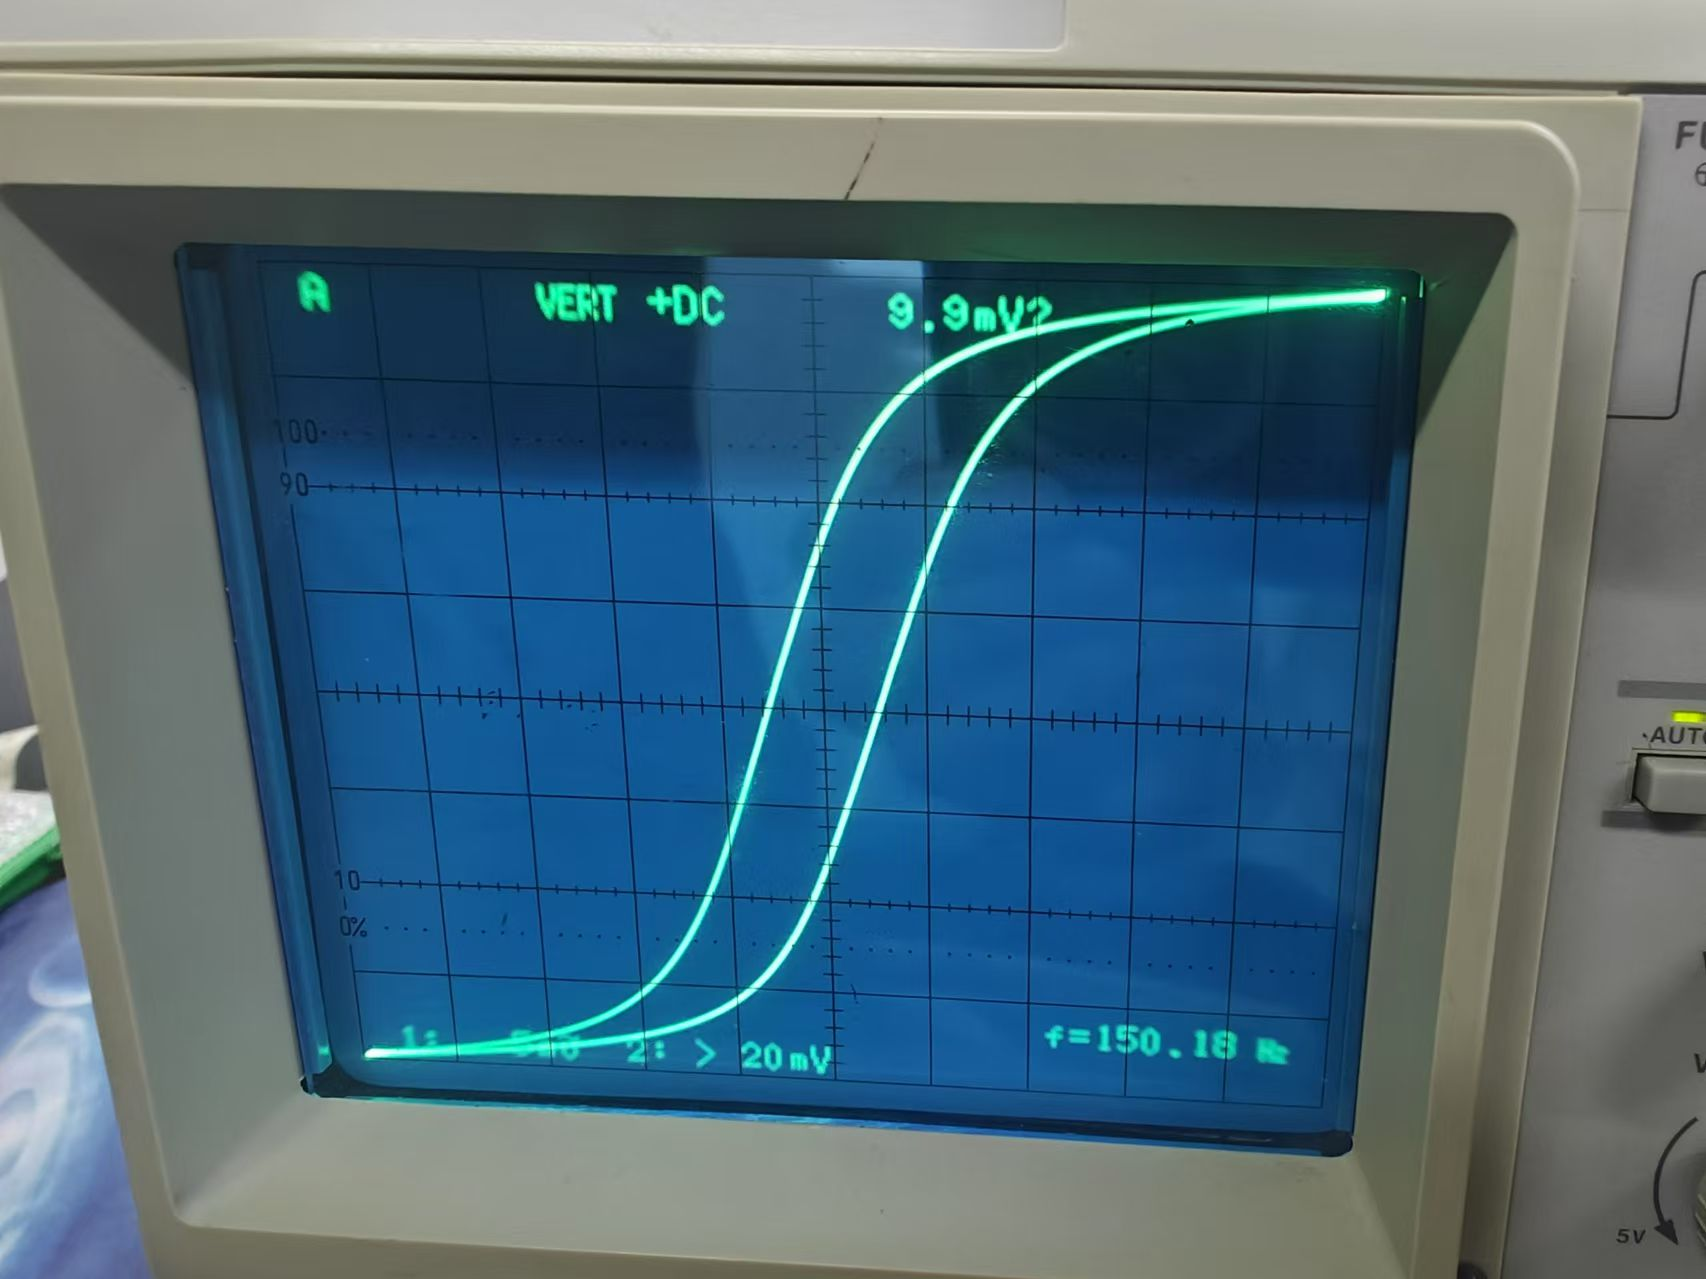
\includegraphics[width=0.7\linewidth]{2.4}
		\caption{150Hz}
		\label{fig:10}
	\end{figure}
	\subsection{基本磁化曲线}
		\begin{table}[H]
		\centering
		\setlength{\extrarowheight}{12pt}  
		\resizebox{0.8\textwidth}{!}{
			\begin{tabular}{|c|c|c|c|c|c|c|c|c|c|c|c|c|}
				\hline
				序号 & 1 & 2 & 3 & 4 & 5 & 6 & 7 & 8 & 9 & 10 & 11 & 12 \\
				\hline
				X格 & 0 & 0.2 & 0.4 & 0.6 & 0.8 & 1.0 & 1.5 & 2.0 & 2.5 & 3.0 & 4.0 & 5.0 \\
				\hline
				H(A/m) &0.00 & 7.69 & 15.38 & 23.08 & 30.77 & 38.46 & 57.69 & 76.92 & 96.15 & 115.38 & 153.85 & 192.31\\
				\hline
				Y(格) &0.00 & 4.80 & 11.60 & 20.80 & 30.60 & 43.50 & 58.40 & 68.40 & 74.20 & 77.80 & 79.60 & 80.40\\
				\hline
				B(mT) & 0.00 & 23.23 & 56.13 & 100.65 & 148.06 & 210.48 & 282.58 & 330.97 & 359.03 & 376.45 & 385.16 & 389.03\\
				\hline
			\end{tabular}
		}
	\end{table}
	\begin{figure}[H]
		\centering
		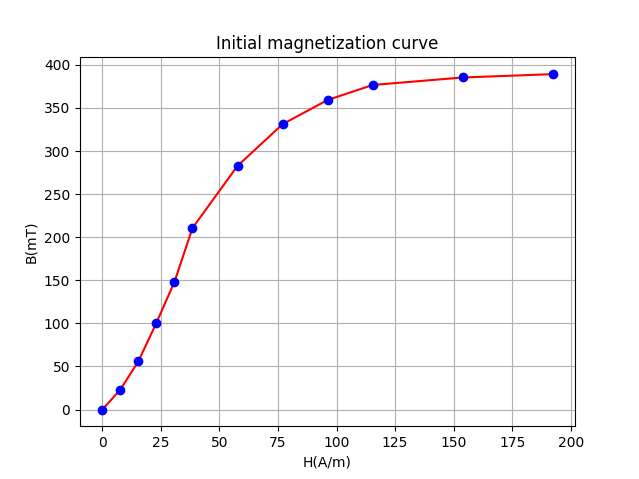
\includegraphics[width=0.7\linewidth]{e}
		\caption{起始磁化曲线}
		\label{fig:11}
	\end{figure}
	
	\subsection{$\mu_2$}
	\begin{figure}[H]
		\centering
		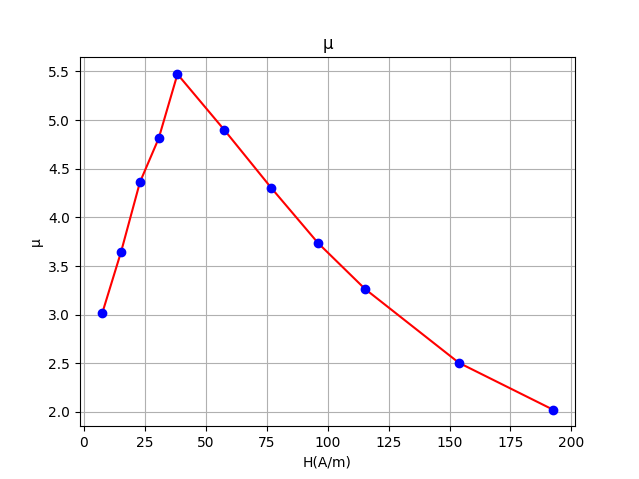
\includegraphics[width=0.7\linewidth]{µ2}
		\caption{}
		\label{fig:u2}
	\end{figure}
	
	\subsection{磁滞回线}
	\begin{tabular}{|c|c|c|c|c|c|c|c|c|c|c|c|c|}
		\hline
		序号 & 1 & 2 & 3 & 4 & 5 & 6 & 7 & 8 & 9 & 10 & 11 & 12 \\
		\hline
		X(格) & -5.00 & -4.00 & -3.00 & -2.50 & -2.00 & -1.50 & -1.00 & -0.80 & -0.60 & -0.40 & -0.20 & 0.00 \\
		\hline
		H(A/m) &  -192.31 & -153.85 & -115.38 & -96.15 & -76.92 & -57.69 & -38.46 & -30.77 & -23.08 & -15.38 & -7.69 & 0.00 \\
		\hline
		Y1(格) &-3.99 & -3.89 & -3.86 & -3.65 & -3.30 & -2.45 & -0.90 & -0.23 & 0.37 & 1.18 & 1.86 & 2.18  \\
		\hline
		Y2(格） &-3.99 & -3.98 & -3.97 & -3.88 & -3.77 & -3.60 & -3.39 & -3.22 & -3.08 & -2.76 & -2.56 & -2.18 \\
		\hline
		B1(mT） &-386.13 & -376.45 & -373.55 & -353.23 & -319.35 & -237.10 & -87.10 & -22.26 & 35.81 & 114.19 & 180.00 & 210.97   \\
		\hline
		B2(mT) &-386.13 & -385.16 & -384.19 & -375.48 & -364.84 & -348.39 & -328.06 & -311.61 & -298.06 & -267.10 & -247.74 & -210.97\\
		\hline
		X(格） &0.00 & 0.20 & 0.40 & 0.60 & 0.80 & 1.00 & 1.50 & 2.00 & 2.50 & 3.00 & 4.00 & 5.00
		\\
		\hline
		H(A/m) &0.00 & 7.69 & 15.38 & 23.08 & 30.77 & 38.46 & 57.69 & 76.92 & 96.15 & 115.38 & 153.85 & 192.31 \\
		\hline
		Y1(格） &2.18 & 2.57 & 2.80 & 3.01 & 3.23 & 3.34 & 3.54 & 3.71 & 3.80 & 3.91 & 3.99 & 4.02  \\
		\hline
		Y2(格） & -2.18 & -1.60 & -0.73 & -0.25 & 0.48 & 1.03 & 2.59 & 3.24 & 3.65 & 3.82 & 3.98 & 4.02\\
		\hline
		B1(mT） &210.97 & 248.71 & 270.97 & 291.29 & 312.58 & 323.23 & 342.58 & 359.03 & 367.74 & 378.39 & 386.13 & 389.03
		\\
		\hline
		B2(mT) & -210.97 & -154.84 & -70.65 & -24.19 & 46.45 & 99.68 & 250.65 & 313.55 & 353.23 & 369.68 & 385.16 & 389.03
		\\
		\hline
	\end{tabular}
	\begin{figure}[H]
		\centering
		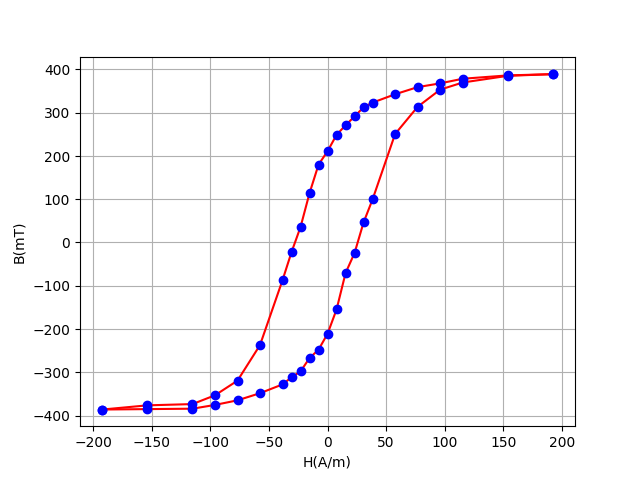
\includegraphics[width=0.7\linewidth]{d}
		\caption{磁滞回线}
		\label{fig:12}
	\end{figure}
	$\mu$
\end{document}